
\section{Validation}
\label{repl:sec:validation}

\LSEQ est une fonction d'allocation d'identifiants pour les structures de
données sans resolution de conflits conçue pour les séquences.  Cette section a
deux objectifs. Tout d'abord, elle examine la contribution de chacun des
composants internes à \LSEQ décrits en §\ref{repl:sec:proposal}.  Ensuite, elle
valide expérimentalement les analyses en complexité de \LSEQ faites en
§\ref{repl:sec:complexity}.

\subsection{Référence}

\begin{figure}
  \begin{center}
    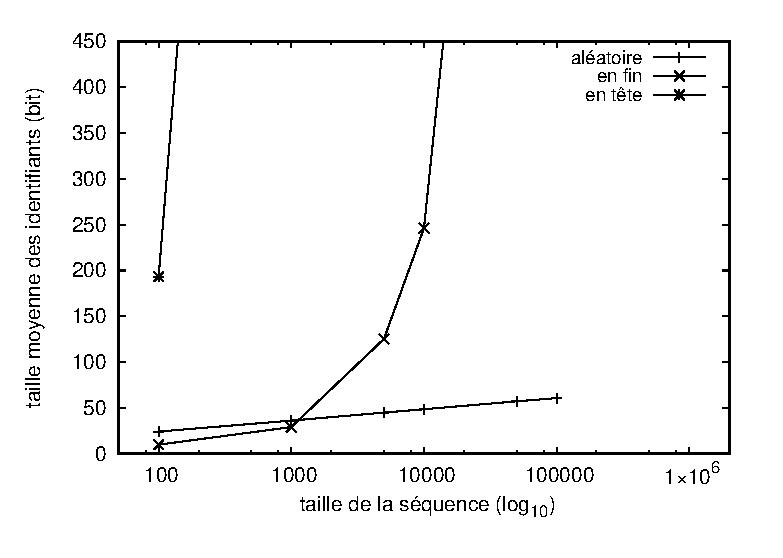
\includegraphics[width=0.8\textwidth]{img/lseq/logoot.eps}
    \caption{\label{repl:img:logoot} Arbre à arité constante avec stratégie
      d'allocation adaptée à l'édition en fin. L'axe des abscisses montre la
      taille du document sur une échelle logarithmique en base décimale. L'axe
      des ordonnées montre la moyenne des tailles des chemins alloués.}
  \end{center}
\end{figure}


\paragraph{Objectif :} Fournir une référence aux futures expérimentations afin
de montrer les améliorations et les dégradations de chaque composant.

\paragraph{Description :} La simulation concerne trois documents artificiels
remplis respectivement par un comportement d'édition aléatoire, un comportement
d'édition monotone de gauche à droite, et un comportement d'édition monotone de
droite à gauche. La fonction d'allocation utilise un arbre d'arité maximale
constante et une seule sous-fonction d'allocation conçue pour l'édition monotone
de gauche à droite. Cette configuration correspond aux stratégies de l'état de
l'art~\cite{preguica2009commutative, weiss2009logoot}.  La moyenne de la taille
des identifiants est mesurée à 100, 1k, 5k, 10k, 50k, 100k insertions.

\paragraph{Résultat :} La figure~\ref{repl:img:logoot} montre les résultats de
cette expérimentation. Nous observons tout d'abord que la taille des
identifiants croît logarithmiquement dans le cas des éditions faites à des
positions aléatoires. Ensuite, les comportements d'édition monotone conduisent
tout deux à une croissance linéaire. Toutefois, l'édition de gauche à droite
reste bien plus efficace que l'édition de droite à gauche.

\paragraph{Explication :} Le comportement d'édition aléatoire conduit à une
structure d'arbre équilibrée. Les identifiants alloués restent petits. Le
comportement d'édition montone de gauche à droite conduit à une croissance
linéaire mais relativement faible. En effet, la stratégie d'allocation employée
est conçue pour ce comportement : Des branches sont laissées disponibles en vue
des prochaines insertions. La taille des identifiants grandit donc
lentement. Toutefois, comme l'arité maximale de l'arbre reste constante, la
structure ne s'adapte pas à la taille du document, d'où la croissance
linéaire. Dans le cas du comportement d'édition monotone de droite à gauche,
l'augmentation de la taille des identifiants est très forte car la stratégie
employée favorise le comportement d'édition opposé. Ainsi les insertions ont tôt
fait de ne plus avoir d'espace disponible conduisant à la création d'un nouvel
espace, i.e. la profondeur de l'arbre augmente. L'augmentation reste linéaire.

\subsection{Arbre exponentiel}

\begin{figure}
  \centering
  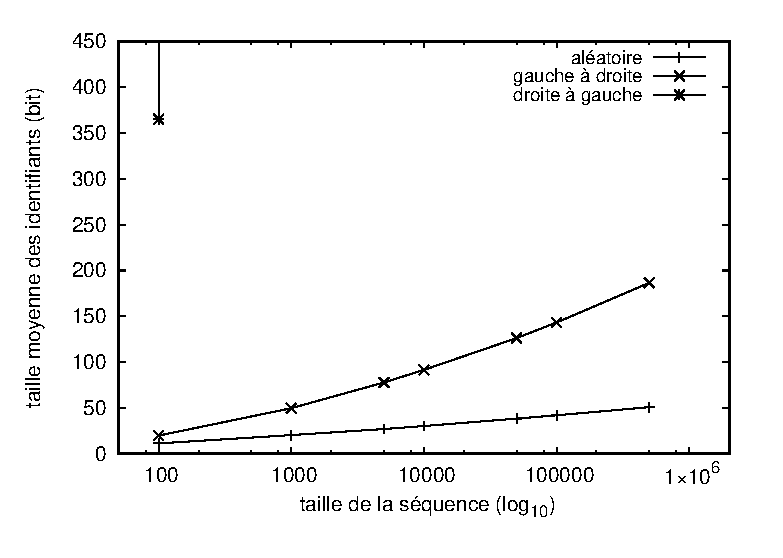
\includegraphics[width=0.8\textwidth]{img/lseq/double.eps}
  \caption{\label{repl:img:exponentialtree} Arbre exponentiel avec stratégie
    d'allocation adaptée à l'édition en fin. L'axe des abscisses montre la
    taille du document sur une échelle logarithmique en base décimale. L'axe des
    ordonnées montre la moyenne des tailles des chemins alloués.}
\end{figure}

\paragraph{Objectif :} Montrer que le chemin des identifiants alloués progresse
de manière sous-linéaire par rapport à la taille du document. Montrer que
lorsque le comportement d'édition va à l'opposé de celui prévu, l'allocation
devient désastreuse.

\paragraph{Description :} Des documents sont créés artificiellement par
insertions successives de caractères. Trois types de comportement d'édition sont
simulés :
\begin{inparaenum}[(i)]
\item à des positions aléatoire dans le document,
\item à la fin,
\item en tête.
\end{inparaenum}
La moyenne de la taille des identifiants est mesurée à 100, 1k, 5k, 10k, 50k,
100k, 500k insertions. La structure utilisée est celle d'un arbre exponentiel
dont l'arité maximale de départ est fixée à $2^5$.

\paragraph{Résultat :} La figure~\ref{repl:img:exponentialtree} montre les
résultats des mesures effectuées pendant la simulation. Nous observons que lors
de l'édition en position aléatoire, l'allocation se comporte extrêmement bien
avec des chemins de taille logarithmique. Lors de l'édition en fin, la taille
moyenne des chemins suit une augmentation sous-linéaire par rapport au nombre
d'insertions dans le document. Finalement, l'édition en tête entraine une très
forte augmentation de la taille des identifiants.

\paragraph{Explication :} L'édition aléatoire place les éléments au hazard dans
la séquence. L'arbre est équilibré car nulle branche n'est remplie en
particulier. À terme, toutes les branches les plus basses sont remplies. Dans ce
cas, les chemins sont de taille moyenne logarithmiques ce qui constitue la borne
minimale. Lors de l'édition en queue, les chemins les plus à gauche sont alloués
réservant de l'espace aux insertions futures. De plus, puisque l'arité de
l'arbre double à chaque niveau, il peut accueillir deux fois plus de chemins à
un prix minime (+1 bit/niveau). Pour cette même raison, l'allocation est
désastreuse lors de l'édition en tête : Quelques insertions suffisent à faire
augmenter la profondeur de l'arbre. L'arité maximale augmente alors rapidement
et le prix des identifiants explose.


\subsection{Sous-fonctions d'allocation}

\begin{figure}
  \centering
  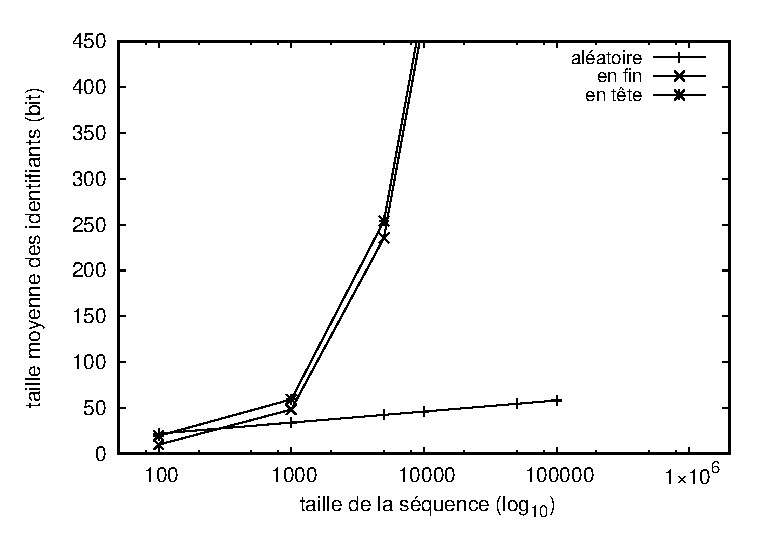
\includegraphics[width=0.8\textwidth]{img/lseq/robin.eps}
  \caption{\label{repl:img:suballocation} Arbre à arité constante et deux
    sous-stratégies d'allocation. L'axe des abscisses montre la taille du
    document sur une échelle logarithmique en base décimale. L'axe des ordonnées
    montre la moyenne des tailles des chemins alloués.}
\end{figure}

\paragraph{Objectif :} Montrer que deux sous-fonctions d'allocation conçues avec
des objectifs antagonistes mais utilisées ensemble gèrent les comportements
d'édition triviaux. Montrer que la progression des identifiants reste linéaire
comparé à la taille du document.

\paragraph{Description :} La simulation concerne trois documents grossissant au
rythme des opérations d'insertions effectuées respectivement en tête, en fin, et
aléatoirement. L'arbre a une arité maximale constante. Chaque niveau se voit
attribuer une sous-fonction d'allocation, i.e., les niveaux pairs avec une
fonction adaptée à l'édition en tête, et les niveaux impairs avec une fonction
adaptée à l'édition en fin. Nous mesurons la moyenne des chemins composant les
identifiants à 100, 1k, 5k, 10k, 50k, 100k insertions.

\paragraph{Résultat :} La figure~\ref{repl:img:suballocation} montre les
résultats obtenus à la suite de ces simulations. Nous observons tout d'abord que
les chemins reste logarithmique sous un comportement d'édition aléatoire. Nous
observons aussi que pour l'édition en tête et l'édition en fin, la progression
est linéaire mais surtout, quasiment identique dans les deux cas.

\paragraph{Explication :} Tout comme pour la
figure~\ref{repl:img:exponentialtree}, l'édition à des positions aléatoire à
pour effet d'équilibrer l'arbre représentant le document répliqué. Les chemins
résultant de ce comportement grandissent de manière logarithmique. Grâce à une
alternance des sous-fonctions d'allocation, la taille des chemins alloués lors
de l'édition en tête ou en fin augmente lentement. Malgré tout, la progression
reste linéaire. De plus, elle augmente deux fois plus rapidement que sans cette
alternance avec un comportement d'édition favorable. En effet, dans le cas de
ces simulations, un niveau sur deux composant un chemin est perdu car consommé
trop vite : la sous-fonction d'allocation assignée à ce niveau n'était pas celle
conçue pour le comportement d'édition courant.


\subsection{Arbre exponentiel et sous-fonctions}

\begin{figure}
  \begin{center}
    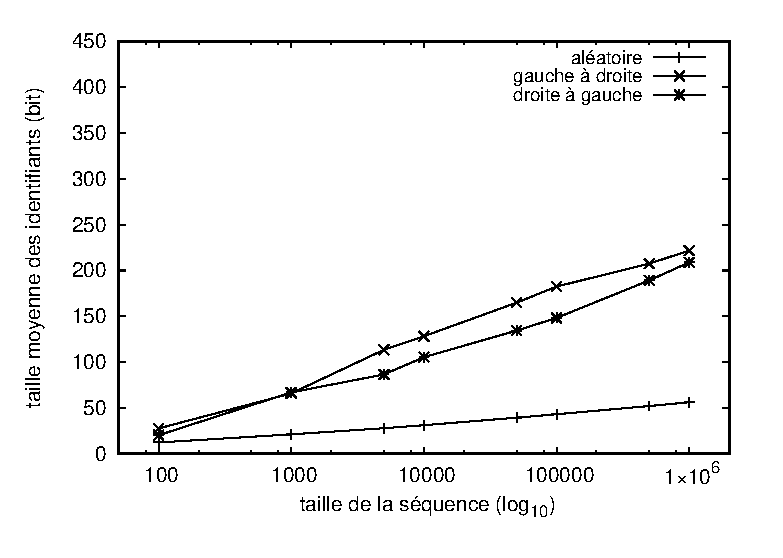
\includegraphics[width=0.8\textwidth]{img/lseq/lseq.eps}
    \caption{\label{repl:img:lseq} Arbre exponentiel avec deux sous-stratégies
      d'allocation. L'axe des abscisses montre la taille du document sur une
      échelle logarithmique en base décimale. L'axe des ordonnées montre la
      moyenne des tailles des chemins alloués.}
  \end{center}
\end{figure}


\subsection{Complexité temporelle}

\begin{figure}
  \begin{center}
    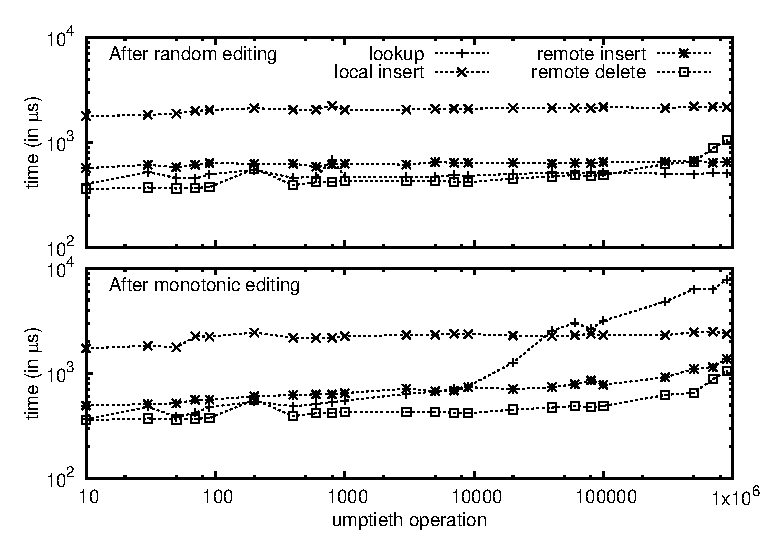
\includegraphics[width=0.8\textwidth]{img/lseq/time.eps}
    \caption{\label{repl:img:time} Performances de la énième opération effectuée
      sur \LSEQ. L'axe des abscisses montre le numéro de la énième
      opération. L'axe des ordonnées montre le temps d'exécution de l'opération
      en microsecondes. La figure du haut considère une structure remplie par
      des insertions aléatoires. La figure du bas considère une structure
      remplies par insertions montones.}
  \end{center}
\end{figure}

\paragraph{Objectif :} Confirmer l'analyse en complexité temporelle de
\LSEQ. Des performances passant à l'echelle sont attendues.

\paragraph{Description :} Cette expérience implique un utilisateur artificiel
unique effectuant des opérations sur sa réplique du document. Le banc d'essai
s'est déroulé sur un \emph{MacBook Pro} comportant un processeur \emph{2.5 GHz
  Intel Core i5}, la version 4.1.1 de \emph{Node.js}, sur une architecture
Darwin 64-bit. Pour chaque opération, un document de $I-1$ caractères est créé
artificiellement. Les mesures s'effectuent sur la $I$\up{ème} opération. Les
opérations prises en compte sont la fonction \textsc{lookup}, la partie locale
de l'insertion, la partie distante de l'insertion, et la partie distante de la
suppression -- la partie locale de cette dernière ne comprend que la propagation
de l'identifiant ciblé aux autres membres. Les mesures sont effectués à
plusieurs reprises sur deux types de documents. Tout d'abord, un document généré
par un comportement d'édition aléatoire, i.e., l'arbre \LSEQ est
équilibré. Ensuite, un document généré par un comportement d'édition monotone,
i.e., une seule branche de l'arbre \LSEQ est remplie. Nous nous intéressons aux
tendences plutôt qu'aux valeurs absolues. En effet, le langage \emph{Javascript}
opère de nombreuses optimisations à la volée. Afin de montrer la contribution
réelle de chacune des opérations, ces optimisations ont été limité au
maximum. Les performances réelles des opérations sont donc nettement meilleures
que celles présentes dans cette expérimentation.

\paragraph{Résultat :} La figure~\ref{repl:img:time} montre les résultats de
cette expérimentation. Nous observons que les valeurs mesurées, dans le cadre
d'un arbre remplies par des éditions aléatoires, ne croissent pratiquement pas,
et ce, quelle que soit l'opération. D'un autre coté, lorsque l'insertion locale
après édition monotone reste stable, nous observons une croissance linéaire du
temps d'exécution de la fonction \textsc{lookup}, et une plus faible évolution
pour les parties distantes des opérations d'insertion et de suppression.

\paragraph{Explication :} Après un comportement d'édition aléatoire, l'arbre de
\LSEQ est équilibré. Par conséquent l'influence d'une opération se limite à un
petit sous ensemble d'éléments composant le document. Par exemple, la fonction
\textsc{lookup} n'a pas besoin d'explorer chaque élément de l'arbre. Elle rejète
rapidement de nombreuses branches sans importances à chaque niveau de l'arbre
car l'indice recherché ne tombe pas dans leur intervalle. Toutefois, cette
remarque n'est pas vraie en ce qui concerne un arbre rempli par un comportement
d'édition monotone. En effet, dans ce cas, la plupart des éléments sont
localisés dans l'une -- et la plus profonde -- des branches de l'arbre. Ainsi,
la fonction \textsc{lookup} va probablement explorer tous les niveaux et
inspecter chaque élément pour en compter le nombre de fils afin d'actualiser son
indice de progression courant. Les mesures concernant les opérations distantes
suivent le même raisonnement. Elles sont plus efficaces car l'exploration des
niveaux utilise la recherche dichotomique.


%%% Local Variables:
%%% mode: latex
%%% TeX-master: "../../paper"
%%% End:
